
\subsection{Fuzzy C-Means}

We have initially tested 216 different configurations of the Fuzzy C-Means (FCM) algorithm on each dataset varying the hyperparameters between the following values:

\begin{itemize}
  \item $n\_clusters$: 2, 3, 4, 5, 7, 9, 11, 13, 15
  \item $m$ (Fuzziness): 1.5, 2, 3, 4, 5, 6, 7, 9
  \item $ \rho $: 0.5, 0.7, 0.9
\end{itemize}

We tried the following stop rules:
\begin{enumerate}
	\item \( \text{max\_iter} \): 100, 300, 500
	\item \( \text{error} \): 1e-1, 1e-4, 1e-5
\end{enumerate}


For each configuration, we ran the algorithm 10 times to mitigate the effects of initialization randomness, resulting in a total of 2160 runs of the FCM algorithm per dataset. From the evaluation metrics extracted in these runs, we analyze the impact of the key hyperparameters and derive insights.

We decided not to include \textit{max\_iter} and \textit{error tolerance} in the analysis of performance metrics, as they do not significantly affect the performance, aside from removing outliers with really bad performance due to a bad inizialization and slightly improving execution time. To illustrate this, we include 3 heatmaps displaying execution times for each dataset, along with the distribution of ARI results for different values of \textit{max\_iter} and \textit{error tolerance} (see \textbf{Figure}\ref{fig:error-iter-fuzzy}).

\begin{figure}[H]
    \centering
    \begin{subfigure}{0.32\textwidth}
        \centering
        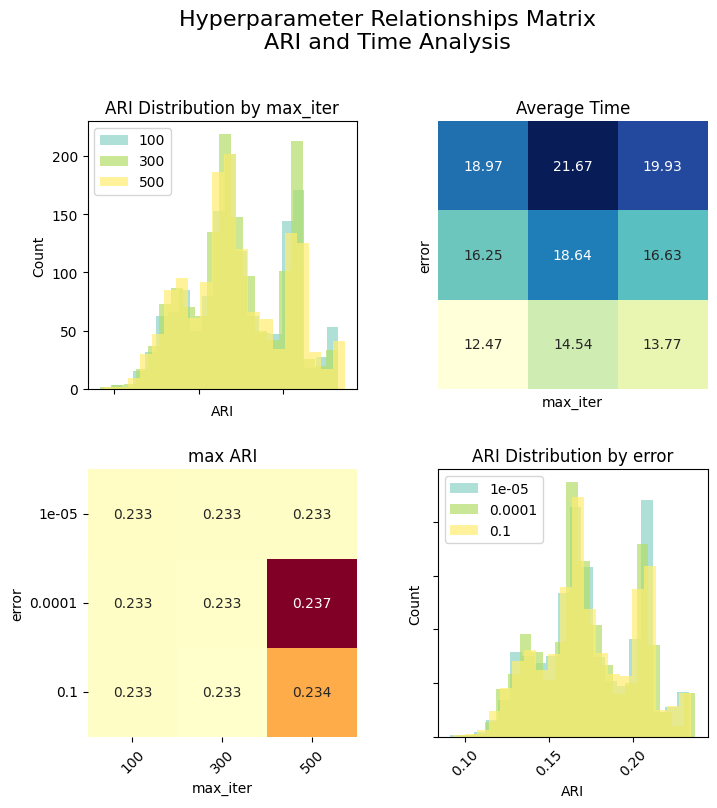
\includegraphics[width=\linewidth]{figures/FuzzyCMeans/penBased_error_iter_pairplot.png}
        \caption{Pen-based dataset.}
    \end{subfigure}
    \begin{subfigure}{0.32\textwidth}
        \centering
        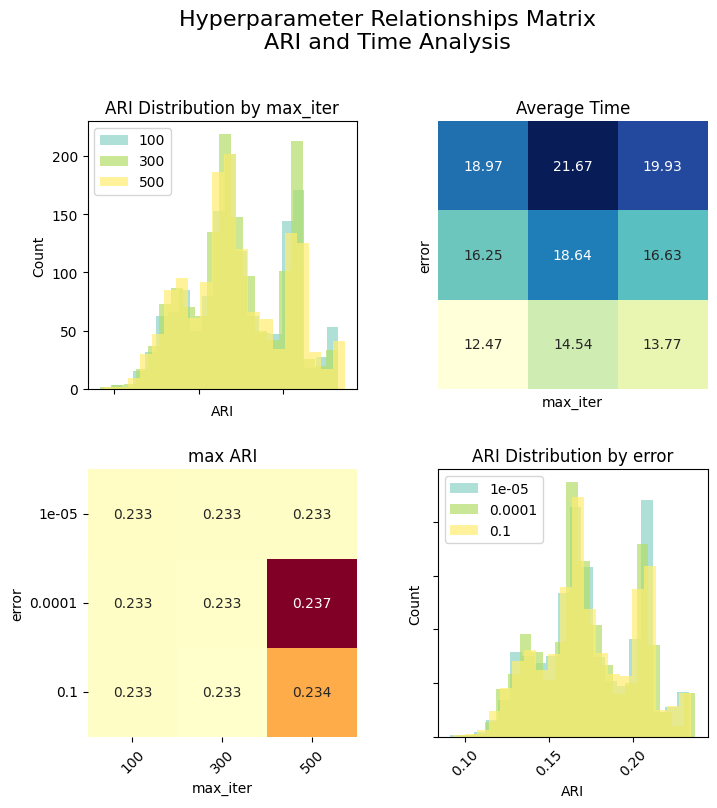
\includegraphics[width=\linewidth]{figures/FuzzyCMeans/mushroom_error_iter_pairplot.png}
        \caption{Mushroom dataset.}
    \end{subfigure}
    \begin{subfigure}{0.32\textwidth}
        \centering
        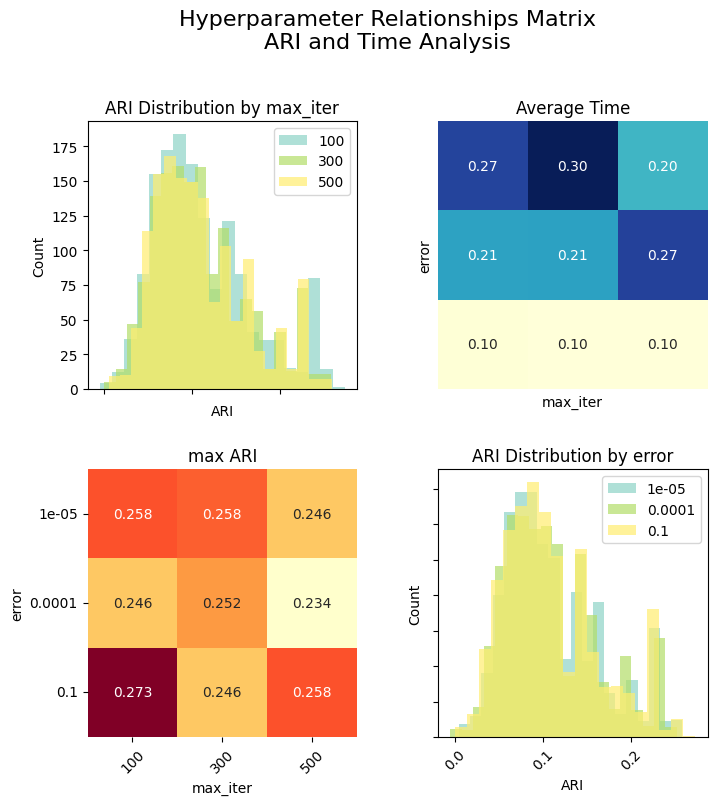
\includegraphics[width=\linewidth]{figures/FuzzyCMeans/hepatitis_error_iter_pairplot}
        \caption{Hepatitis dataset.}
    \end{subfigure}
    \caption{Heatmaps illustrating execution times for each dataset, showcasing performance across different configurations.}
    \label{fig:error-iter-fuzzy}
\end{figure}


\subsubsection{Preliminary Study}

We first explored preliminary patterns in the measured metrics and the influence of hyperparameters on clustering performance.


\textbf{Figure} \ref{fig:metrics_corr_fuzzy} illustrates the relationships between the various metrics for the FCM algorithm. Similar trends to the ones observed in K-means (see \textbf{Figure} \ref{fig:metrics_corr}): (1) \textbf{External metrics} (\textit{ARI}, \textit{NMI}) are highly correlated as both improve when the clusters assimilates to the ground truth. (2) Regarding \textbf{internal metrics}, \textit{Silhouette} and \textit{CHS} are negatively correlated with \textit{DBI}, probably because the first two metrics measure cluster cohesion and separation positively, while \textit{DBI} assesses the ratio of intra-cluster dispersion to inter-cluster separation, where lower \textit{DBI} values indicate better clustering quality.

\begin{figure}[H]
	\centering
	\begin{subfigure}{0.32\textwidth}
		\centering
		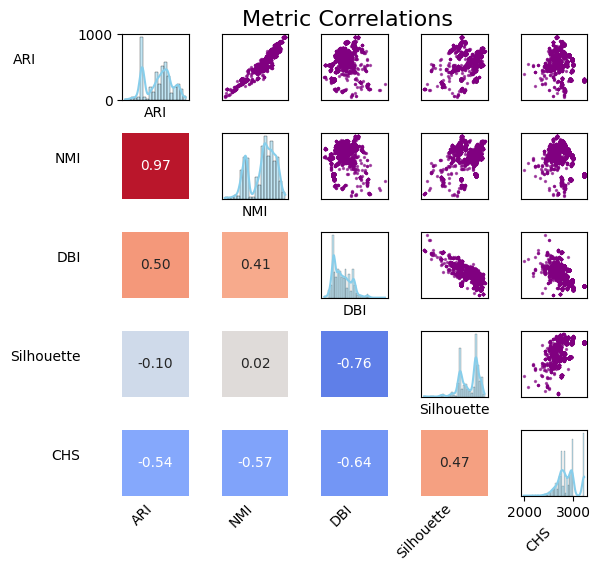
\includegraphics[width=\linewidth]{figures/FuzzyCMeans/penBased_metrics_correlations_matrix.png}
		\caption{Pen-based dataset.}
	\end{subfigure}
	\begin{subfigure}{0.32\textwidth}
		\centering
		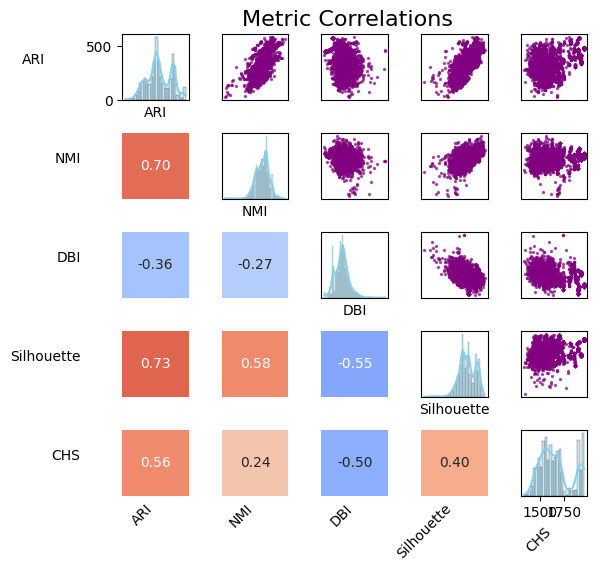
\includegraphics[width=\linewidth]{figures/FuzzyCMeans/mushroom_metrics_correlations_matrix.png}
		\caption{Mushroom dataset.}
	\end{subfigure}
	\begin{subfigure}{0.32\textwidth}
		\centering
		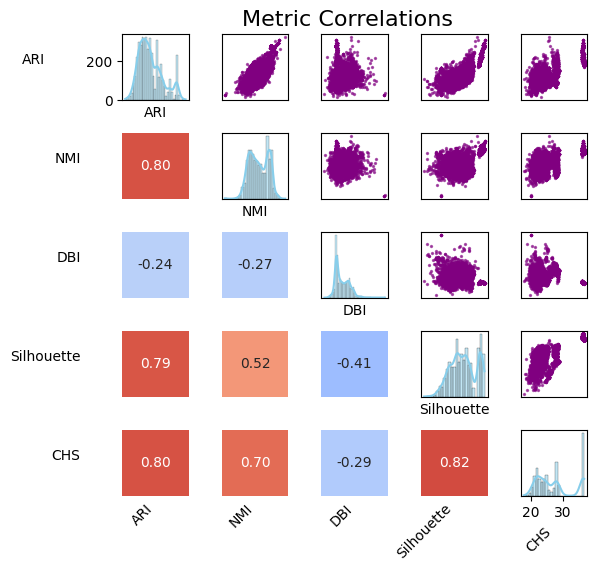
\includegraphics[width=\linewidth]{figures/FuzzyCMeans/hepatitis_metrics_correlations_matrix.png}
		\caption{Hepatitis dataset.}
	\end{subfigure}
	\caption{Metrics correlation acrross the three datasets.}
	\label{fig:metrics_corr_fuzzy}
\end{figure}

Additionally, Figure \ref{fig:heatmaps_grid_comparison_fuzzy} illustrates pairwise relationships between hyperparameters, specifically the impact of fuzziness ($m$), the number of clusters (\texttt{n\_clusters}), and the generalized parameter ($\rho$) on clustering quality (evaluated using the maximum value) and execution time (evaluated using the average). The following conclusions can be drawn from these plots:

\begin{itemize} \item \textbf{General Observations}: \begin{enumerate} \item An increase in computation time is observed with higher values of \textit{n\_clusters}, \textit{fuzziness} ($m$), or $\rho$. This aligns with the understanding that a higher number of clusters, increased fuzziness, or a lower quasi-learning rate (inversely related to $\rho$) slows convergence. \item Variations in $\rho$ do not significantly affect the ARI metric, as $\rho$ is primarily intended to accelerate the method's convergence rather than enhance clustering performance. \end{enumerate} \item \textbf{Dataset-Specific Insights}: \begin{enumerate} \item For datasets with fewer classes (e.g., Hepatitis and Mushroom), clustering performance improves with a smaller number of clusters, whereas datasets like Pen-Based benefit from higher values of \textit{n\_clusters}. \item Lower fuzziness ($m$) yields better performance for sparse datasets (e.g., Mushroom and Hepatitis), which have high dimensionality relative to the number of instances. Conversely, higher fuzziness appears advantageous for dense datasets like Pen-Based, where cluster boundaries are likely less distinct. \end{enumerate} \end{itemize}


\begin{figure}[H]
	\centering
	\adjustbox{max width=\textwidth, max height=\textwidth}{%
		\begin{tabular}{cccc}
			% Row 1: Hepatitis
			\multicolumn{4}{c}{\textbf{Hepatitis Dataset}} \\ 
			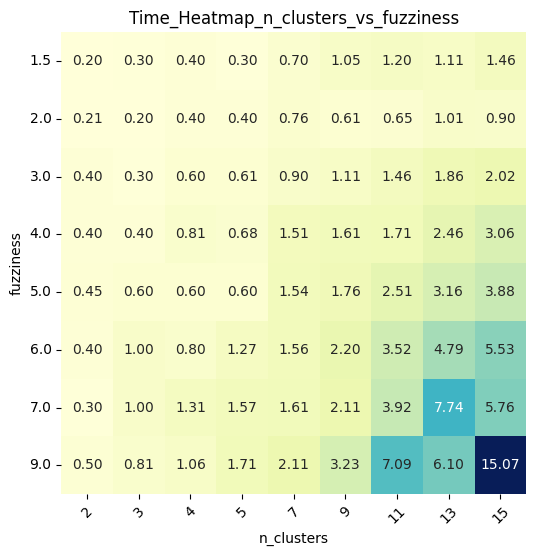
\includegraphics[width=0.23\textwidth]{figures/FuzzyCMeans/Hepatitis/Time_Heatmap_n_clusters_vs_fuzziness.png} &
			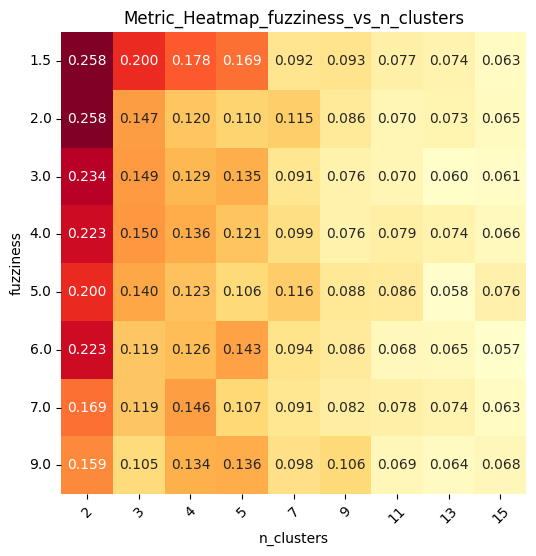
\includegraphics[width=0.23\textwidth]{figures/FuzzyCMeans/Hepatitis/Metric_Heatmap_fuzziness_vs_n_clusters.png} &
			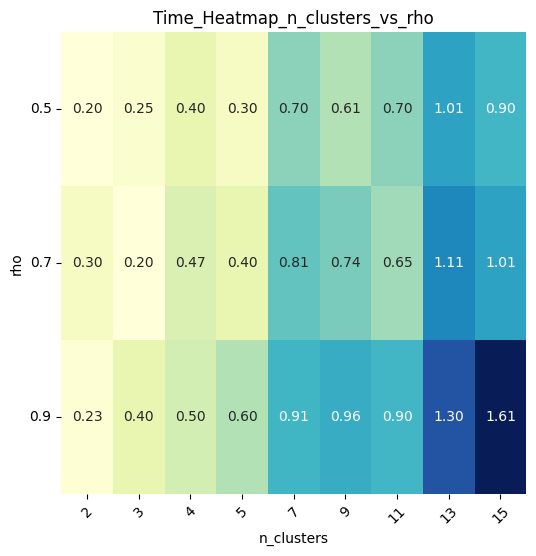
\includegraphics[width=0.23\textwidth]{figures/FuzzyCMeans/Hepatitis/Time_Heatmap_n_clusters_vs_rho.png} &
			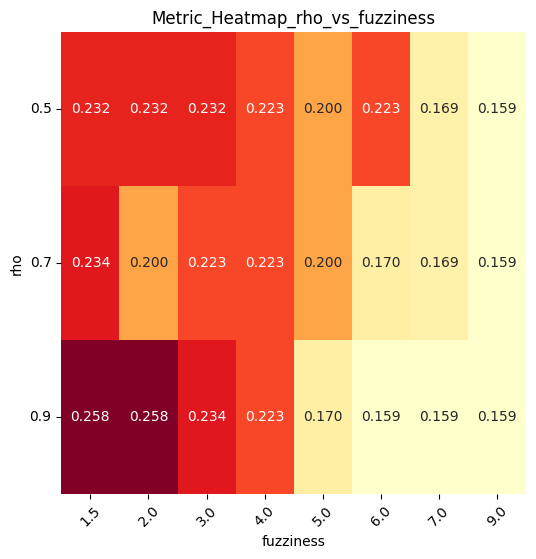
\includegraphics[width=0.23\textwidth]{figures/FuzzyCMeans/Hepatitis/Metric_Heatmap_rho_vs_fuzziness.png} \\[1em]
			
			% Row 2: Mushroom
			\multicolumn{4}{c}{\textbf{Mushroom Dataset}} \\ 
			\includegraphics[width=0.23\textwidth]{figures/FuzzyCMeans/Mushroom/Time_Heatmap_n_clusters_vs_fuzziness.png} &
			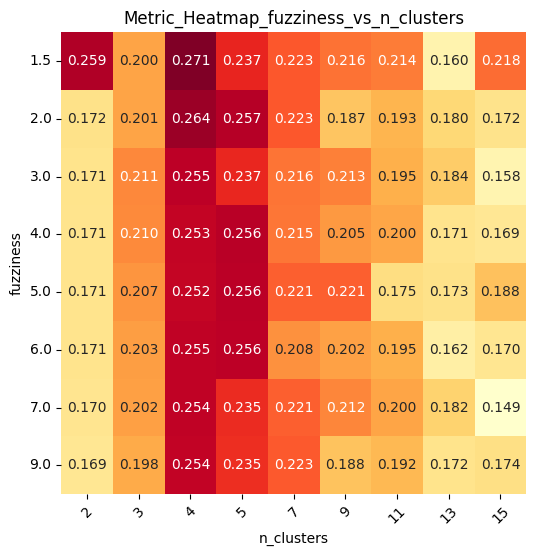
\includegraphics[width=0.23\textwidth]{figures/FuzzyCMeans/Mushroom/Metric_Heatmap_fuzziness_vs_n_clusters.png} &
			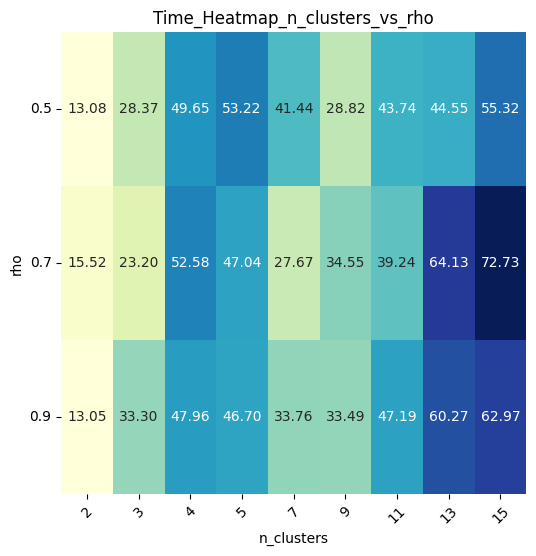
\includegraphics[width=0.23\textwidth]{figures/FuzzyCMeans/Mushroom/Time_Heatmap_n_clusters_vs_rho.png} &
			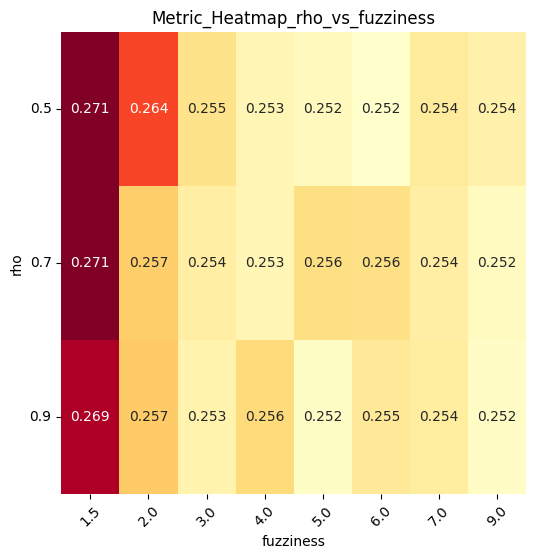
\includegraphics[width=0.23\textwidth]{figures/FuzzyCMeans/Mushroom/Metric_Heatmap_rho_vs_fuzziness.png} \\[1em]
			
			% Row 3: Pen-Based
			\multicolumn{4}{c}{\textbf{Pen-Based Dataset}} \\ 
			\includegraphics[width=0.23\textwidth]{figures/FuzzyCMeans/PenBased/Time_Heatmap_n_clusters_vs_fuzziness.png} &
			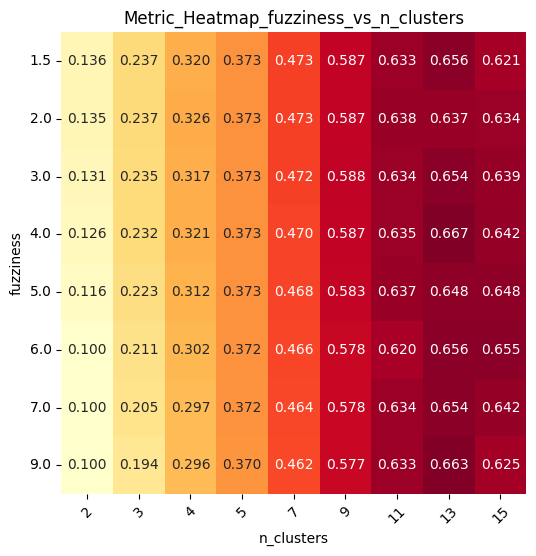
\includegraphics[width=0.23\textwidth]{figures/FuzzyCMeans/PenBased/Metric_Heatmap_fuzziness_vs_n_clusters.png} &
			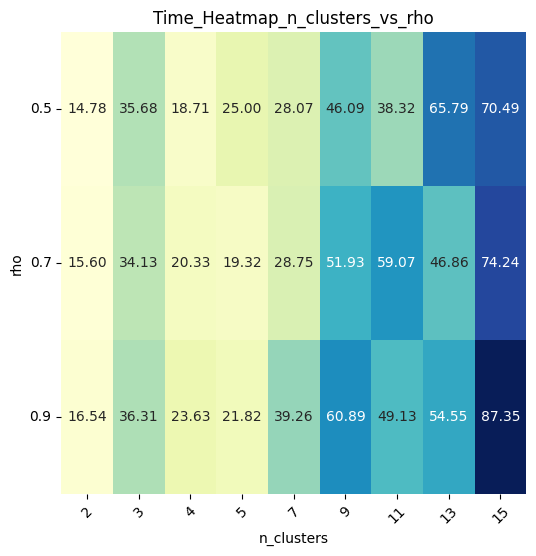
\includegraphics[width=0.23\textwidth]{figures/FuzzyCMeans/PenBased/Time_Heatmap_n_clusters_vs_rho.png} &
			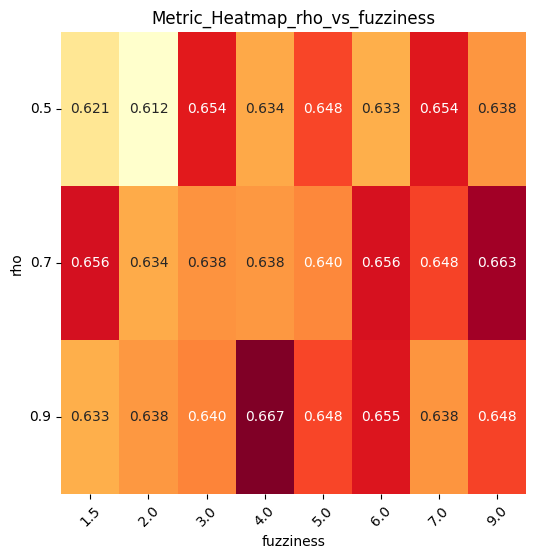
\includegraphics[width=0.23\textwidth]{figures/FuzzyCMeans/PenBased/Metric_Heatmap_rho_vs_fuzziness.png} \\
		\end{tabular}
	}
	\caption{Comparison of heatmaps for Time and Metrics across Hepatitis, Mushroom, and Pen-Based datasets.}
	\label{fig:heatmaps_grid_comparison_fuzzy}
\end{figure}

\subsubsection{Unified Study of Parameters}

To provide a comprehensive understanding of the impact of key parameters (\textit{m} and \texttt{n\_clusters}) on clustering performance, we analyze violin plots for a selection of metrics across the Mushroom, Pen-Based, and Hepatitis datasets. These plots reveal dataset-specific trends that inform optimal parameter selection.

\begin{itemize}
	\item \textbf{Mushroom Dataset:}
	\begin{enumerate}
		\item Silhouette scores reach their highest value at $m=3$, indicating
		that moderately sharp cluster boundaries enhance separability in this
		dataset.
		
		\item Optimal NMI and CHS values are observed at $\texttt{n\_clusters}=2$ and
		$4$, suggesting that the dataset's inherent structure is best
		represented by a smaller number of well-defined clusters.
	\end{enumerate}
	
	\item \textbf{Pen-Based Dataset:}
	\begin{enumerate}
		\item CHS achieves peak performance with moderate \texttt{n\_clusters}
		values (e.g., $3$ and $4$), balancing granularity and overfitting. In contrast, NMI increases steadily with higher \texttt{n\_clusters} values, reflecting alignment with the dataset's true labels.
		
		\item Higher values of \textit{m} result in reduced DBI, indicating improved
		intra-cluster cohesion—a critical factor for datasets with overlapping clusters.
	\end{enumerate}
	
	\item \textbf{Hepatitis Dataset:}
	\begin{enumerate}
		\item DBI consistently improves with increasing \texttt{n\_clusters}, except
		for an initial degradation from $2$ to $3$, highlighting the importance
		of fine-grained clustering to capture the dataset's complexity. NMI peaks
		at $\texttt{n\_clusters}=2$, aligning with the dataset's labeled
		structure.
		
		\item Lower \textit{m} values enhance Silhouette scores, reflecting a preference
		for sharp cluster boundaries to effectively distinguish small and diverse
		groups.
	\end{enumerate}
\end{itemize}

\begin{figure}[H]
	\centering
	\adjustbox{max width=\textwidth, max height=\textheight}{%
		\begin{tabular}{ccc}
			% Row 1: Mushroom
			\multicolumn{3}{c}{\textbf{Mushroom Dataset}} \\ 
			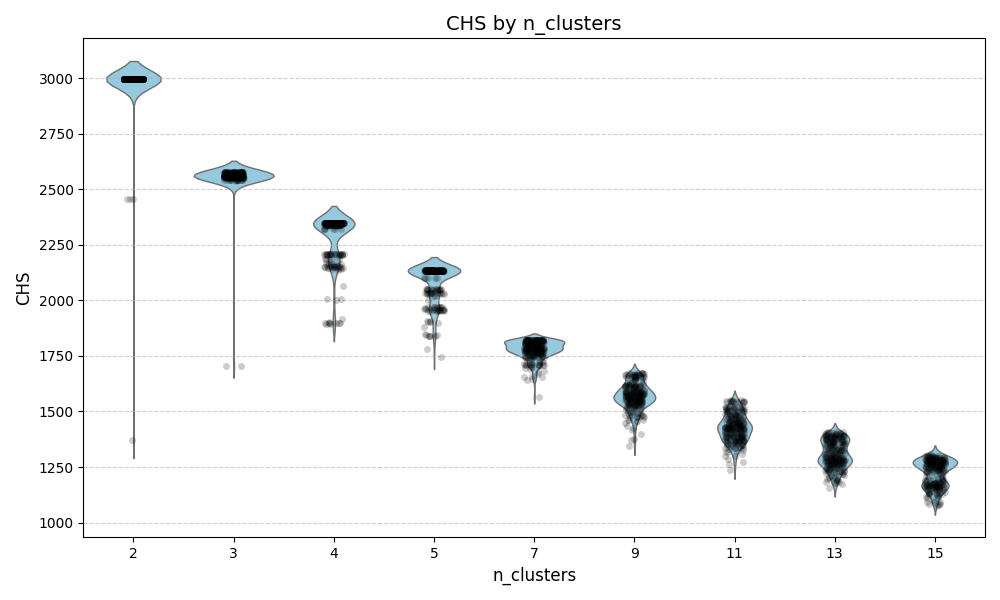
\includegraphics[width=0.30\textwidth]{figures/FuzzyCMeans/Mushroom/violin_n_clusters_vs_CHS.png} &
			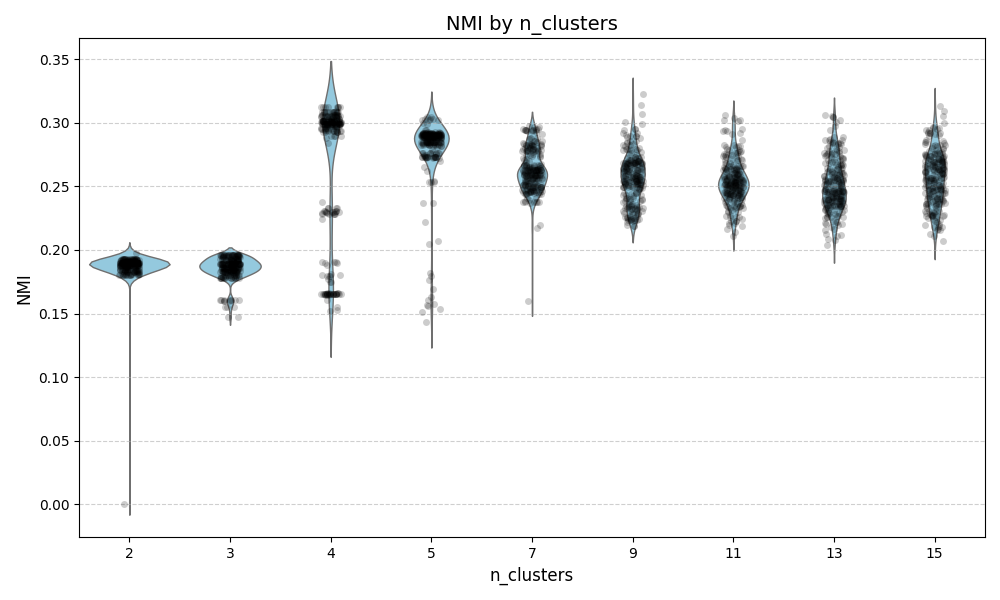
\includegraphics[width=0.30\textwidth]{figures/FuzzyCMeans/Mushroom/violin_n_clusters_vs_NMI.png} &
			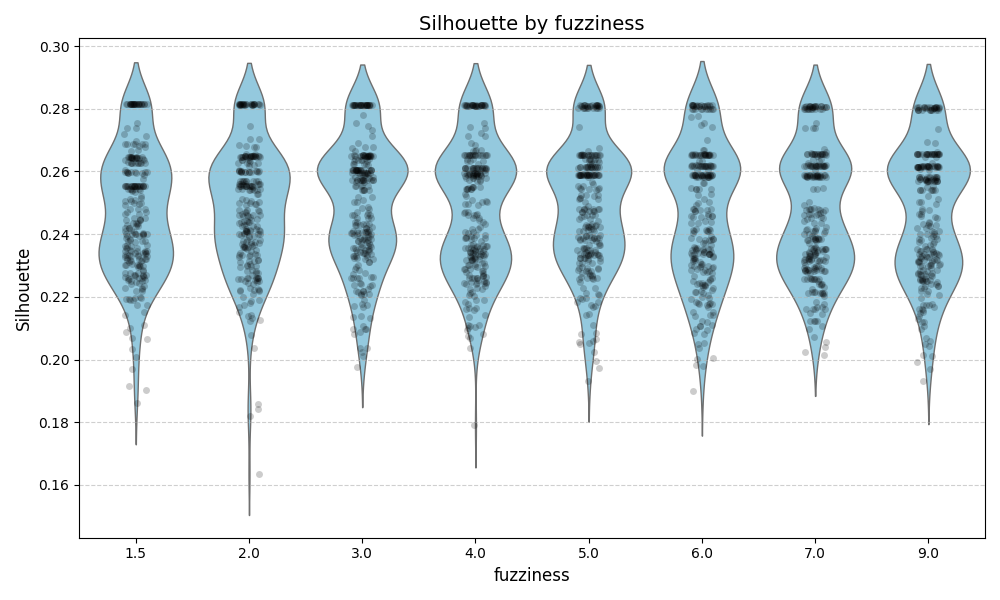
\includegraphics[width=0.30\textwidth]{figures/FuzzyCMeans/Mushroom/violin_fuzziness_vs_Silhouette.png} \\
			
			% Row 2: Pen-Based
			\multicolumn{3}{c}{\textbf{Pen-Based Dataset}} \\ 
			\includegraphics[width=0.30\textwidth]{figures/FuzzyCMeans/PenBased/violin_n_clusters_vs_NMI.png} &
			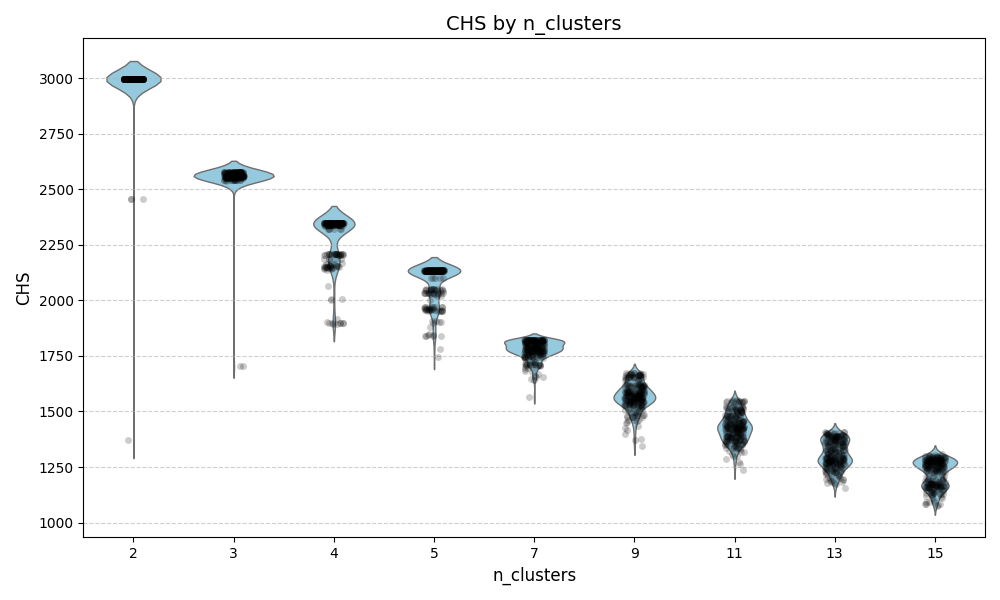
\includegraphics[width=0.30\textwidth]{figures/FuzzyCMeans/PenBased/violin_n_clusters_vs_CHS.png} &
			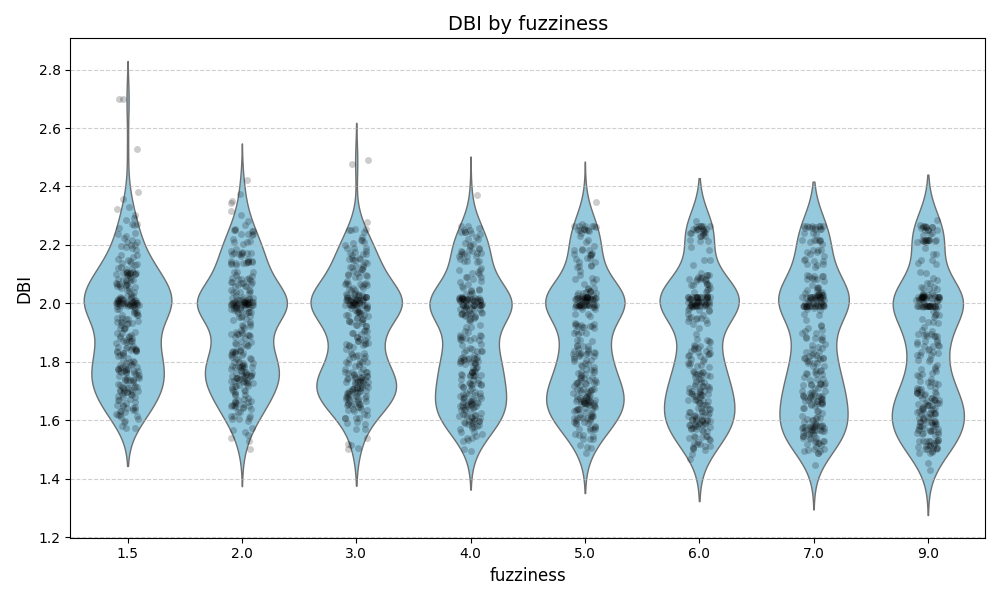
\includegraphics[width=0.30\textwidth]{figures/FuzzyCMeans/PenBased/violin_fuzziness_vs_DBI.png} \\
			
			% Row 3: Hepatitis
			\multicolumn{3}{c}{\textbf{Hepatitis Dataset}} \\ 
			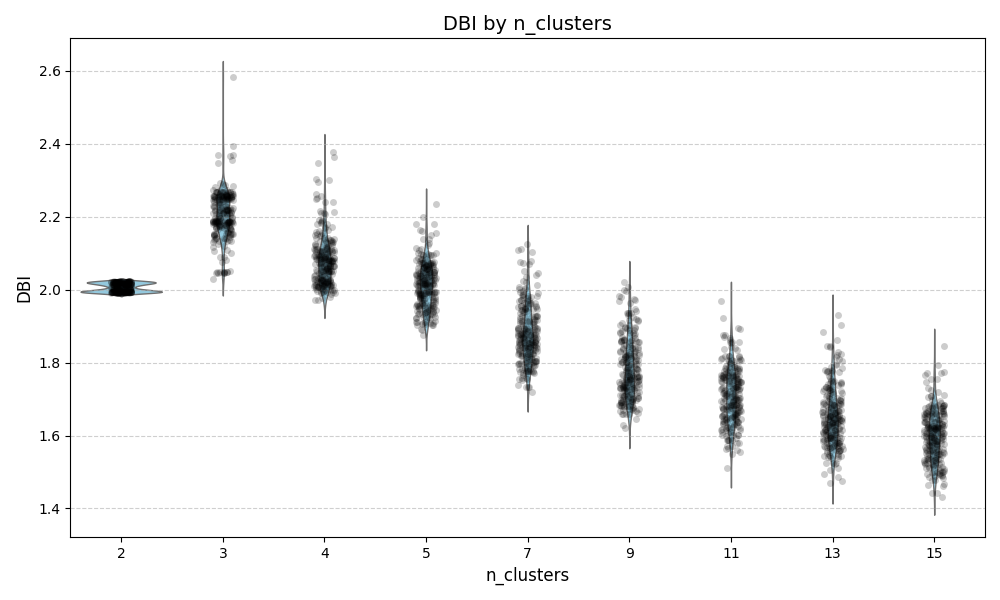
\includegraphics[width=0.30\textwidth]{figures/FuzzyCMeans/Hepatitis/violin_n_clusters_vs_DBI.png} &
			\includegraphics[width=0.30\textwidth]{figures/FuzzyCMeans/Hepatitis/violin_n_clusters_vs_NMI.png} &
			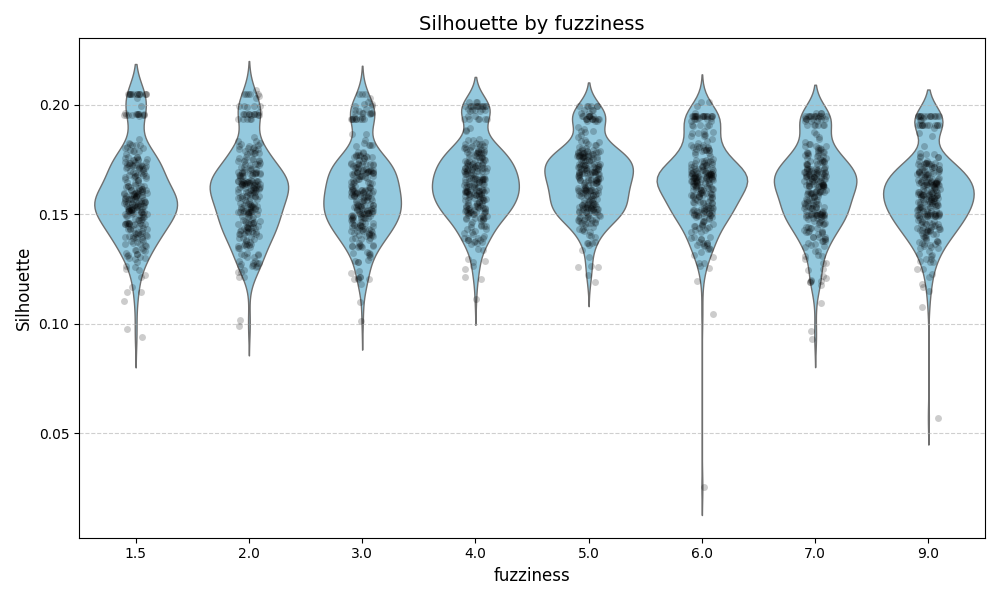
\includegraphics[width=0.30\textwidth]{figures/FuzzyCMeans/Hepatitis/violin_fuzziness_vs_Silhouette.png} \\
		\end{tabular}
	}
	\caption{Violin plots illustrating the effect of \textit{m} (fuzziness) and \texttt{n\_clusters} on various clustering metrics across the Mushroom, Pen-Based, and Hepatitis datasets. Rows represent datasets, while columns depict specific parameter-metric relationships.}
	\label{fig:unified_parameter_study}
\end{figure}

\subsubsection{Best Runs}
For each dataset, we extracted the configuration that achieved the best score for each metric. This results in five sg-FCM configurations per dataset, which we consider the best runs for that dataset (in no particular order). A summary of the best configurations for the three datasets is shown in Table \ref{tab:sgfcm:best_runs}.

\begin{table}[h!]
	\centering
	\begin{tabular}{|c|cccc|cccc|cccc|}
		\hline
		& \multicolumn{4}{c|}{\textbf{Hepatitis}} & \multicolumn{4}{c|}{\textbf{Mushroom}} & \multicolumn{4}{c|}{\textbf{Pen-Based}} \\ \hline
		\textbf{Metric} & \textbf{\texttt{clusters}} & \textbf{\textit{m}} & \textbf{\(\rho\)} & \textbf{Value} & 
		\textbf{\texttt{clusters}} & \textbf{\textit{m}} & \textbf{\(\rho\)} & \textbf{Value} & 
		\textbf{\texttt{clusters}} & \textbf{\textit{m}} & \textbf{\(\rho\)} & \textbf{Value} \\ \hline
		ARI            & 2           & 1.5         & 0.9   & 0.2585 & 
		4           & 1.5         & 0.5   & 0.2708 & 
		13          & 4.0         & 0.9   & 0.6672 \\ \hline
		NMI            & 2           & 1.5         & 0.9   & 0.2222 & 
		9           & 1.5         & 0.7   & 0.3224 & 
		15          & 6.0         & 0.9   & 0.7452 \\ \hline
		DBI            & 15          & 6.0         & 0.9   & 1.4303 & 
		3           & 6.0         & 0.7   & 1.1127 & 
		9           & 7.0         & 0.7   & 1.2040 \\ \hline
		Silhouette     & 2           & 2.0         & 0.9   & 0.2066 & 
		2           & 1.5         & 0.5   & 0.2816 & 
		13          & 3.0         & 0.5   & 0.3290 \\ \hline
		CHS            & 2           & 1.5         & 0.5   & 36.77  & 
		2           & 1.5         & 0.5   & 2996.24 & 
		4           & 1.5         & 0.7   & 3361.04 \\ \hline
	\end{tabular}
	\caption{Best configurations and their corresponding parameter values (\texttt{n\_clusters}, \textit{m}, \(\rho\)) and metric values for sg-FCM across the three datasets.}
	\label{tab:sgfcm:best_runs}
\end{table}

From these results, we can draw several conclusions about the best hyperparameter configurations for sg-FCM:
\begin{enumerate}
	\item \textbf{Hepatitis:} Low values of \texttt{n\_clusters} (2 and 3) dominate the top configurations, reflecting the dataset's small number of distinct classes. Higher values of \textit{m} improve DBI, suggesting better intra-cluster cohesion for fuzzier assignments.
	
	\item \textbf{Mushroom:} The best configurations favor low fuzziness values (\textit{m} = 1.5), which is expected given the dataset's sparse nature. Lower \(m\) values (between 2 and 4) nearer to the ground truth.
	
	\item \textbf{Pen-Based:} Intermediate to high values of \texttt{n\_clusters} (9, 13, and 15) are optimal, consistent with the dataset's real number of classes. Higher values of m improve performance in this dataset as it is more dense than the others.
\end{enumerate}

Additionally, the larger datasets (Mushroom and Pen-Based) achieve better metric values compared to the smaller Hepatitis dataset. Pen-Based performs particularly well across most metrics, reflecting its compatibility with the sg-FCM clustering algorithm. 


\begin{figure}[H]
	\centering
	\begin{subfigure}{0.32\textwidth}
		\centering
		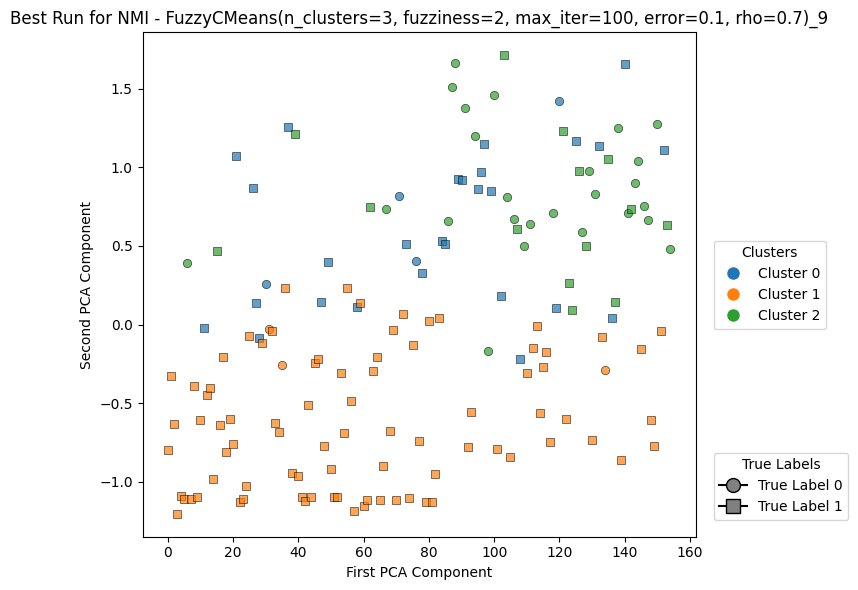
\includegraphics[width=\linewidth]{figures/FuzzyCMeans/Hepatitis/best_run_NMI.png}
		\caption{Hepatitis Dataset (NMI)}
	\end{subfigure}
	\hfill
	\begin{subfigure}{0.32\textwidth}
		\centering
		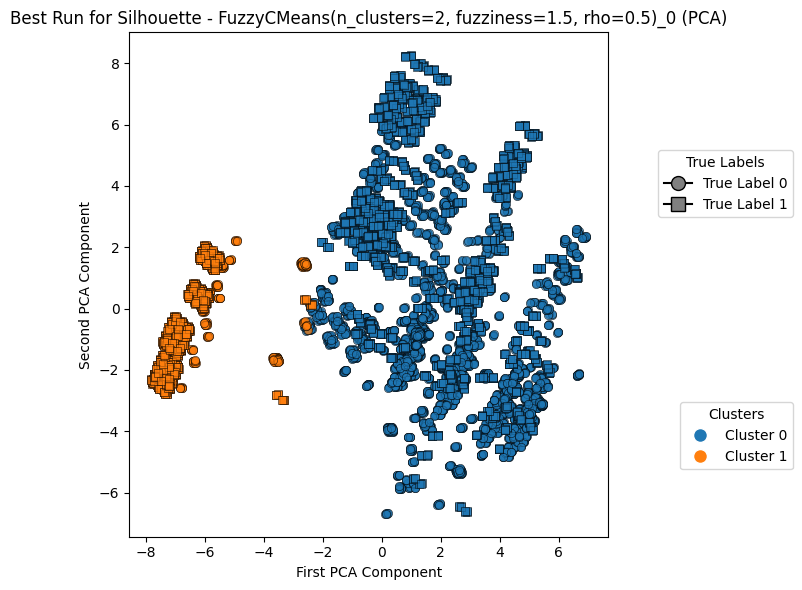
\includegraphics[width=\linewidth]{figures/FuzzyCMeans/Mushroom/best_run_Silhouette.png}
		\caption{Mushroom Dataset (CHS)}
	\end{subfigure}
	\hfill
	\begin{subfigure}{0.32\textwidth}
		\centering
		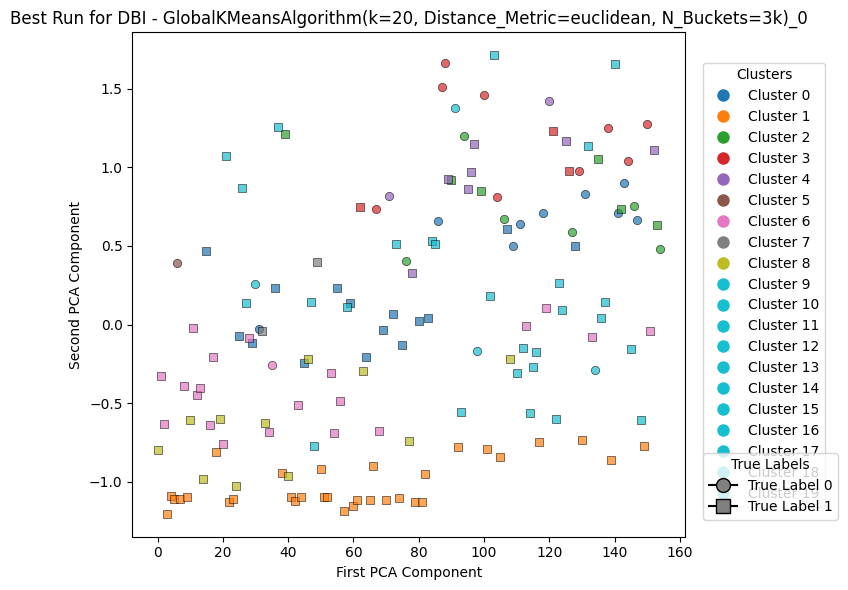
\includegraphics[width=\linewidth]{figures/FuzzyCMeans/PenBased/best_run_DBI.png}
		\caption{Pen-Based Dataset (Silhouette)}
	\end{subfigure}
	\caption{Resulting clusters for each dataset using the best sg-FCM configurations (after PCA).}
	\label{fig:sgfcm:clusters}
\end{figure}
